\documentclass{beamer}
% english language
\usepackage[english]{babel}

% tables
\usepackage{tabularx}
\usepackage{graphicx}
\usepackage{hyperref}
\usepackage{listings}
\usepackage{color}
\usepackage{svg}
\usepackage{xcolor}
\usepackage{algorithm}
\usepackage{algpseudocode}

\usetheme{Madrid}

% unibs color #3d5895
% \definecolor{unibs}{RGB}{61,88,149}
\definecolor{unibs}{HTML}{3d5895}

\definecolor{offset}{HTML}{ff1a1a}
\definecolor{reading_offset}{HTML}{1a40ff}


\setbeamercolor{palette primary}{fg=white, bg=unibs}
\setbeamercolor{palette secondary}{fg=white, bg=unibs}
\setbeamercolor{palette tertiary}{fg=white, bg=unibs}
\setbeamercolor{palette quaternary}{fg=white, bg=unibs}





\title{Exact Cover}
\author{Denis Festa}
\date{\today}

\begin{document}


% \frame{\titlepage}
% Title page with logo
\begin{frame}
    % \centering
    % logo on title page
    \titlepage
    \centering
    
\includegraphics[width=0.2\linewidth]{unibs-circ-logo.pdf}
\end{frame}

% Logo on every slide at the top-right corner
\logo{
\includegraphics[width=0.1\linewidth]{unibs_logo.pdf}}

% \begin{frame}
%     \frametitle{Table of contents}
%     \tableofcontents
% \end{frame}

\section{Introduction}
\begin{frame}
    \frametitle{Introduction}

    The following presentation provides a self-contained report on the 
    implementation of the exact cover problem provided by prof. Marina Zanella
    (University of Brescia, Italy).
    The language of choice is Python for its simplicity and readability.
    The code is available at \url{https://www.kaggle.com/code/denisfesta/exact-cover-problem}.
    The following points discuss:
    \begin{itemize}
        \item the choice of the data structures for the algorithm in its basic form;
        \item the exploration of the solutions to different problems;
        \item the comparison between loading portions of the file and loading the 
            whole file;
        \item the comparison between the basic algorithm and the \textit{plus} 
            algorithm;
        \item the application of the algorithm to the sudoku problem.
    \end{itemize}

\end{frame}

\section*{Data structures}

\begin{frame}
    \frametitle{Data structures}

    To pursue the goal of implementing the algorithm, the matrices A and B need
    to be stored in an appropriate data structure. Since the matrices contain
    only 0s and 1s, the first idea might be to store boolean values instead
    of integers, however, using 
    % True and False written in code style
    \texttt{True} and \texttt{False} gives no advantage.
    One popular library that provides boolean arrays and matrices is
    \texttt{numpy}, which I compare with the less popular \texttt{bitarray}
    library and show the results in figures (\ref{fig:mem_array}) and 
    (\ref{fig:mem_matrix}).
    The elements of a \texttt{numpy} array or matrix occupy less memory than
    the elements of a \texttt{bitarray} array or matrix, however,
    the \texttt{numpy} variable storing the array occupies more memory 
    than the \texttt{bitarray} variable storing the array.
    Given the absence of matrix operations, I don't see any 
    particular advantage in using \texttt{numpy} over \texttt{bitarray}.
    
\end{frame}

\begin{frame}
        % picture "mem_array.png" here
        \begin{figure}
            \centering
            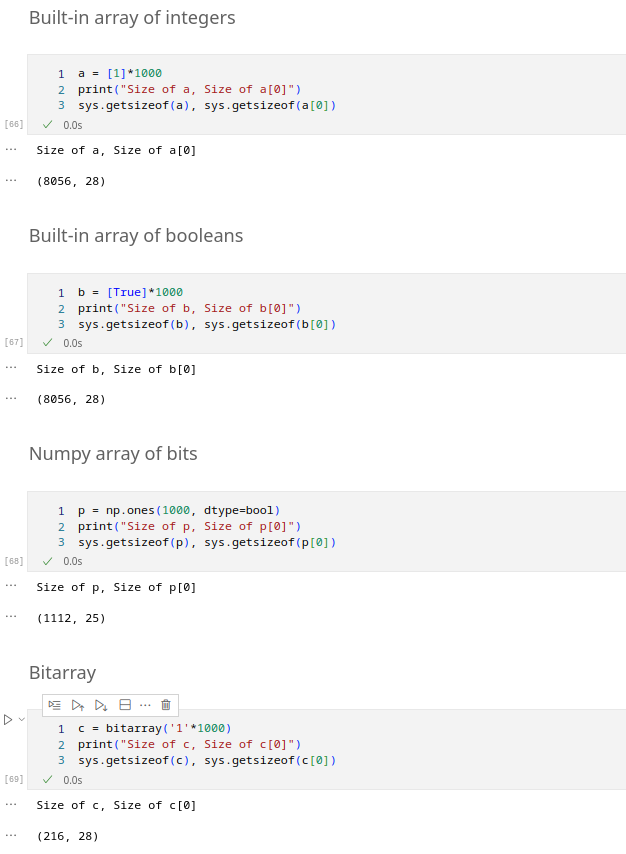
\includegraphics[width=0.6\textwidth]{mem_array.png}
            % \caption{}
            \label{fig:mem_array}
        \end{figure}
\end{frame}

\begin{frame}
        % picture "mem_matrix.png" here
        \begin{figure}
            \centering
            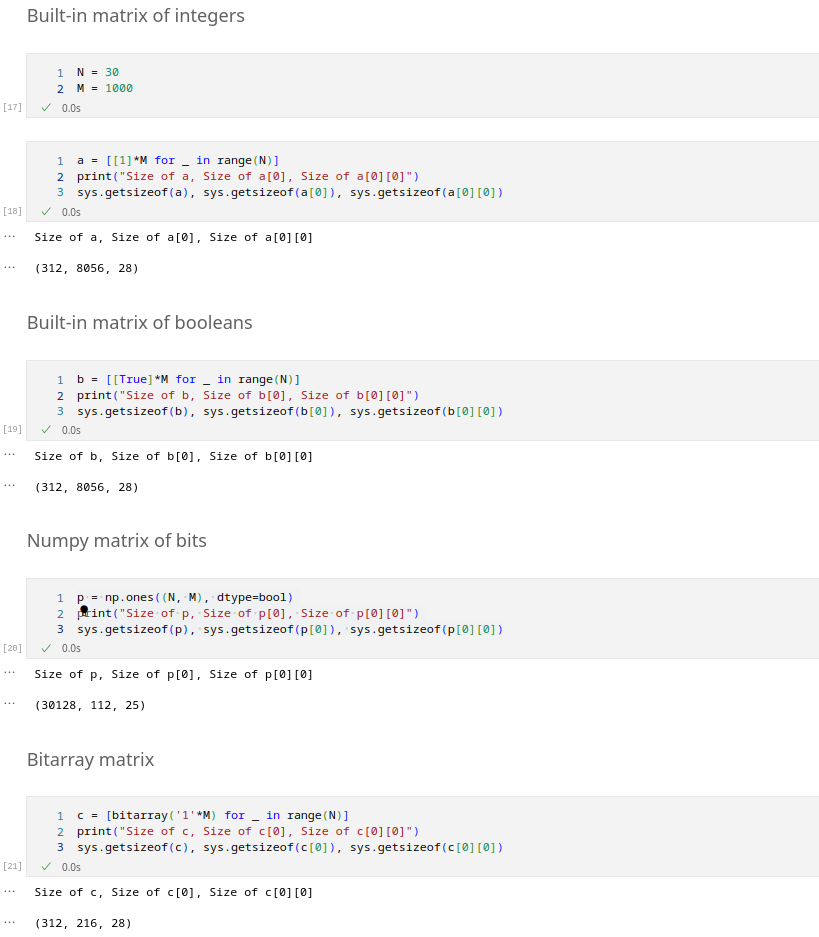
\includegraphics[width=0.55\textwidth]{mem_matrix.png}
            % \caption{}
            \label{fig:mem_matrix}
        \end{figure}
\end{frame}

\begin{frame}
    I tried to profile the code with \texttt{memory-profiler} 
    to find whether the memory occupation
    advantages
    we expect to gain from choosing one data structure over the other
    are actually realized, but I couldn't see any significant difference
    in the memory usage while executing the code, I guess it's because
    the memory required to store the matrices is negligible compared
    to the memory required to store the set of solutions, the set of explored nodes
    and the stack of the recursive calls.
\end{frame}

\section*{Exploring the solutions}

\begin{frame}
    \frametitle{Exploring the solutions}
    Different choices of the cardinality of the domain (columns of the matrix A) and
    the number of sets (rows of the matrix A, rows and columns of the matrix B) 
    lead to different values of:
    \begin{itemize}
        \item the number of solutions found;
        \item the number of explored nodes to find the solutions;
        \item the time required to find the solutions.
    \end{itemize}
    In the following slides I show the values of these quantities for different
    autmatically generated instances of the problem, for time constraints I kept the 
    number of sets in a range between 20 and $\sim400$ and the cardinality of the domain
    in a range between 5 and 14.
\end{frame}

\begin{frame}{Solutions found}
    It's intuitive that the number of solutions found increases
    with the number of sets and decrease with the cardinality of the domain.
    In this case the intuition is confirmed by the solutions found (\ref{fig:sol_5x5}) (at least, those
    found in the chosen dimensions of the problem).
\end{frame}

\begin{frame}
    \begin{figure}
        \centering
        \includegraphics[width=0.6\textwidth]{sol_5x5.pdf}
        % \caption{}
        \label{fig:sol_5x5}
    \end{figure}
\end{frame}

\begin{frame}{Explored nodes}
    It might seem intuitive that, similarly to the previous case, the number of explored nodes
    increases with the number of sets and decreases with the cardinality of the domain,
    however, the same problems that were solved in the previous case display a different
    and less intuitive behaviour in this case (\ref{fig:explored_5x5}).
    The interpretation of this behaviour is that the algorithm has to work harder,
    that is to explore more nodes, to find the solutions for more complex problems, that
    is those problems with a higher number of rows and a higher number of columns.
    Why, fixed the number of rows, a small number of columns implies a higher
    number of explored nodes? I don't know.
\end{frame}

\begin{frame}
    \begin{figure}
        \centering
        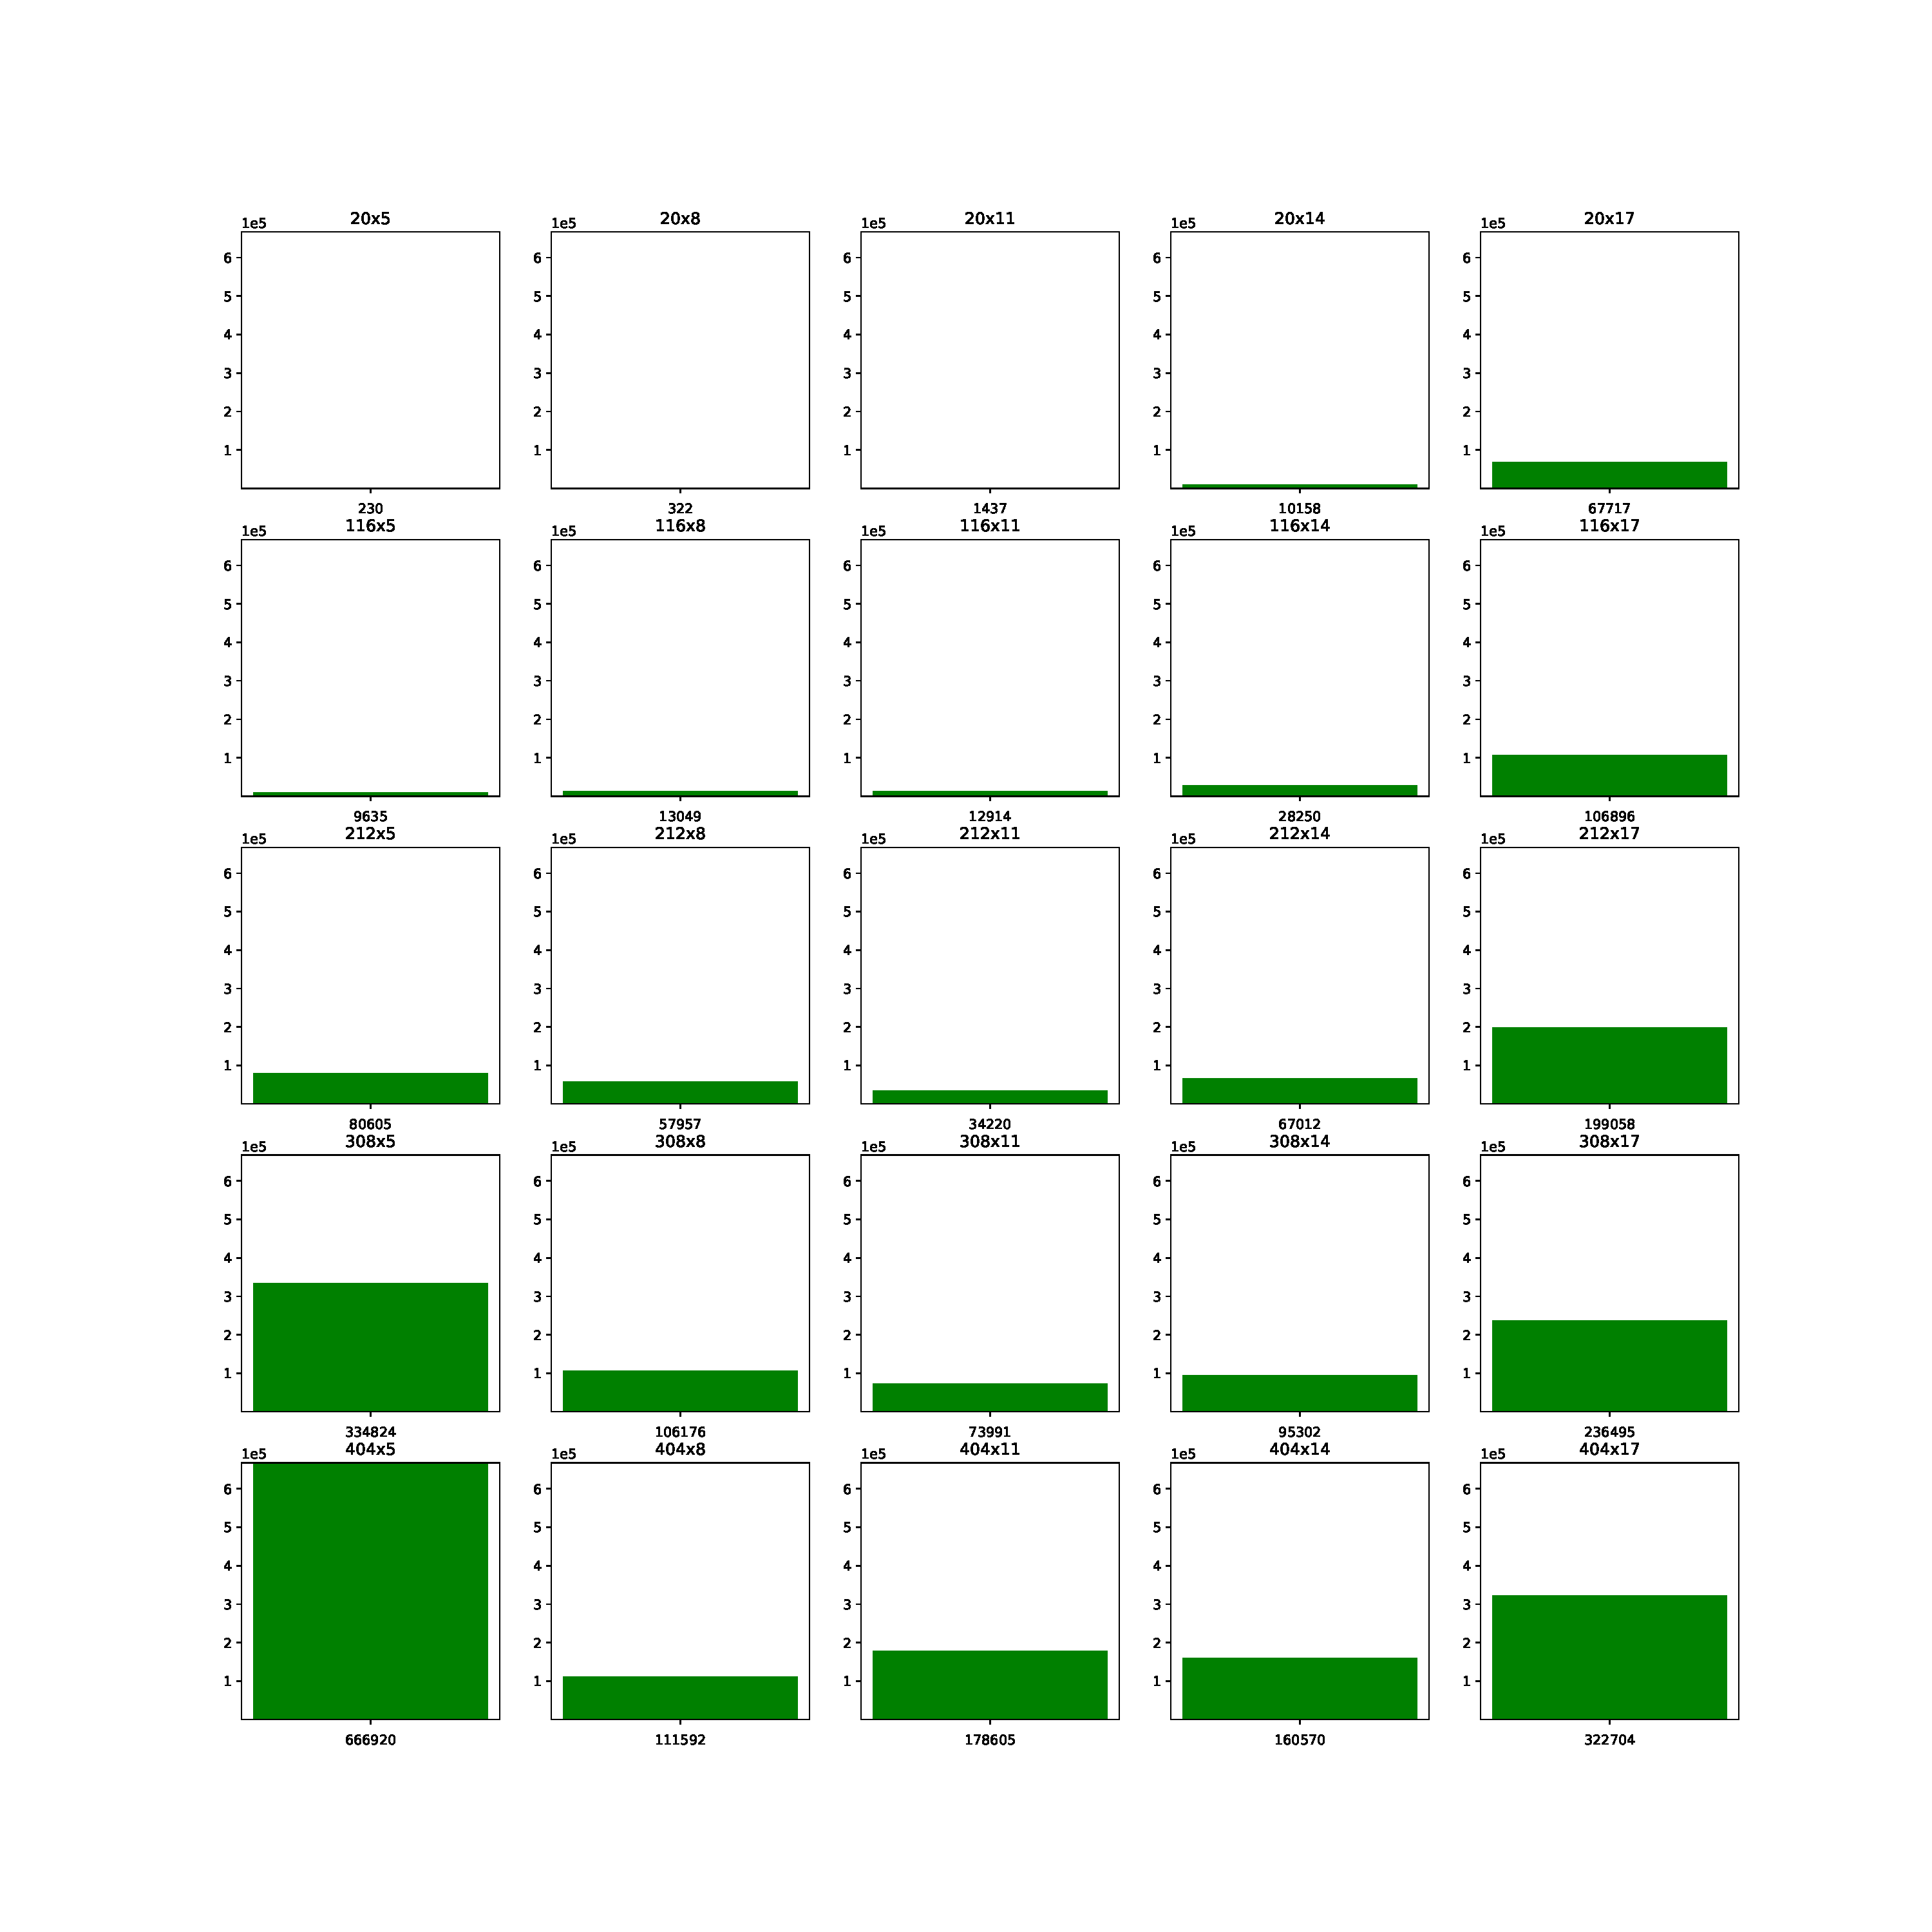
\includegraphics[width=0.6\textwidth]{explored_5x5.pdf}
        % \caption{}
        \label{fig:explored_5x5}
    \end{figure}
\end{frame}

\begin{frame}{Explorable nodes}
    The implemented algorithm chooses to prune the nodes in the tree
    that cannot lead to a plausible solution.
    If the algorithm were to explore all the possible nodes, then for the 
    $i$-th set the number of nodes to explore would be $2^i$,
    hence, if $n$ is the number of sets (rows of A),
    the number of nodes to explore would be $\sum_{i=0}^{n-1} 2^i = 2^n - 1$.

    In figure (\ref{fig:explored_vs_explorable_5x5}) the enormous difference
    between the number of explored nodes and the number of explorable nodes is shown.
    the number of explorable nodes is not exactly $2^n - 1$ because
    the actual computation to represent the explorable nodes is 
    $\sum_{i\in\mathcal{E}}2^i$ where $\mathcal{E}$ is the set of
    explorable  indices
    pointing to rows of A different from an all-zero row (which would be,
    by definition, compatible with any other row).
\end{frame}

\begin{frame}
    \begin{figure}
        \centering
        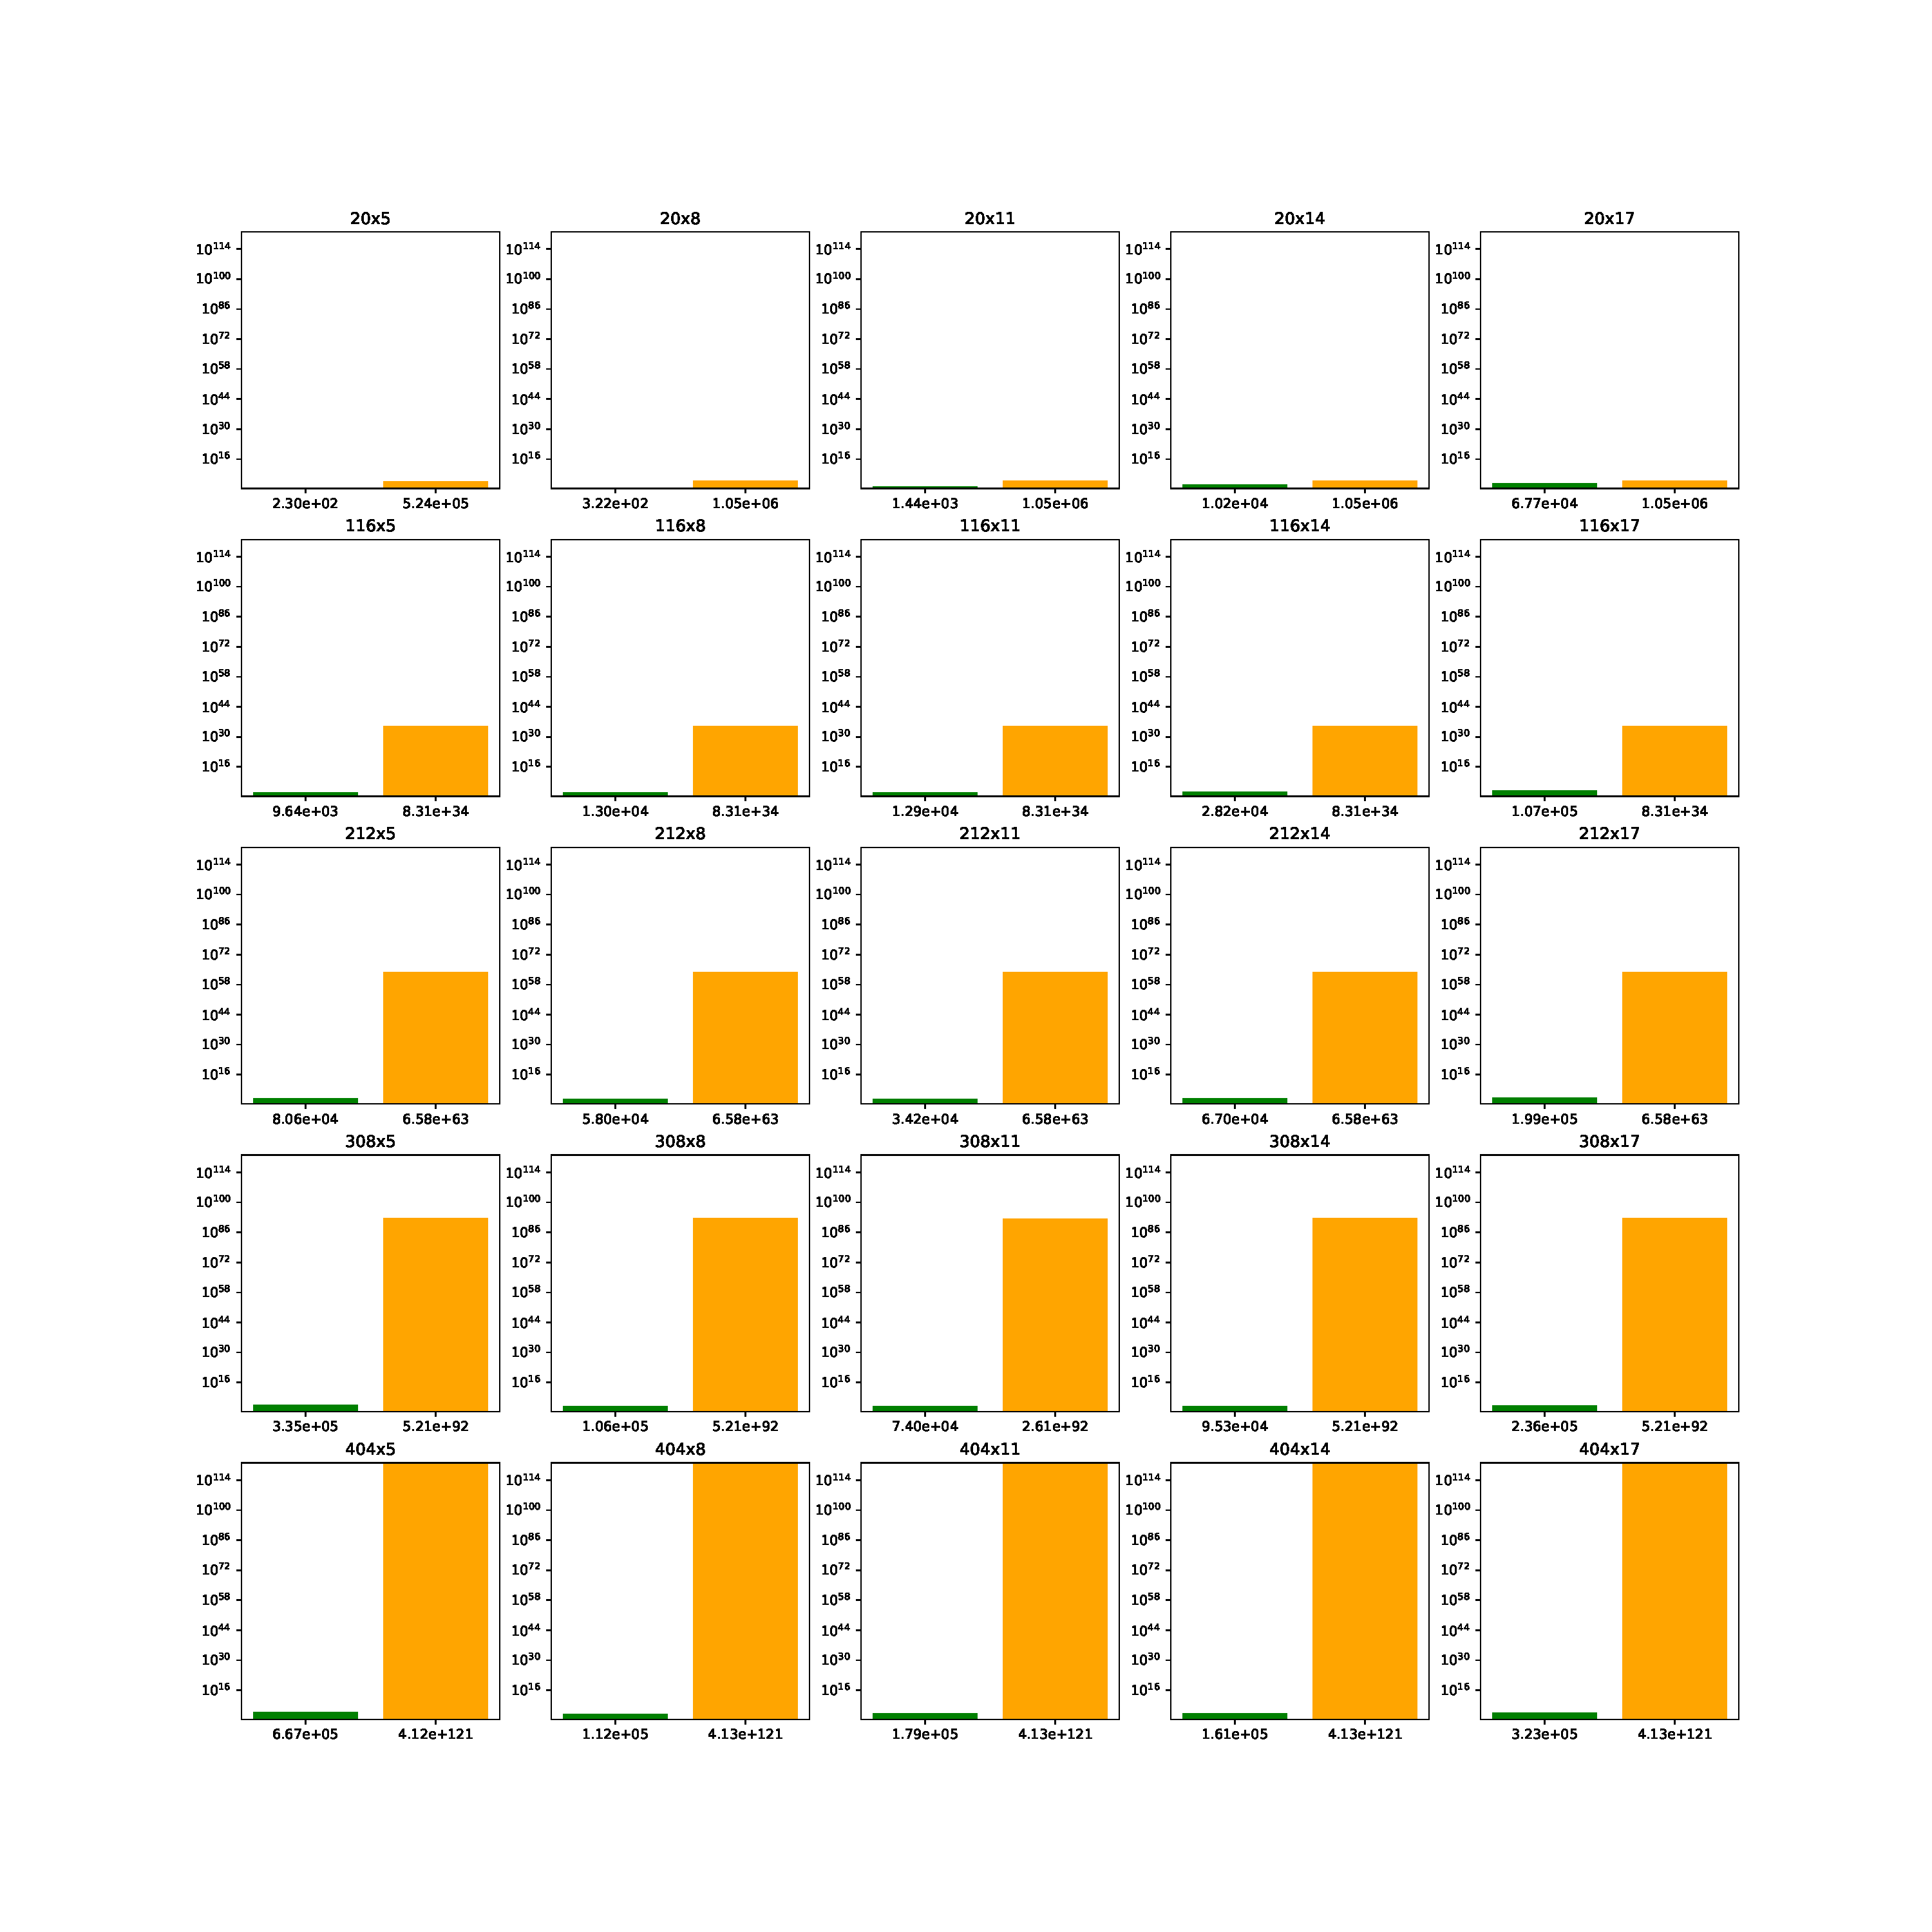
\includegraphics[width=0.6\textwidth]{explored_vs_explorable_5x5.pdf}
        % \caption{}
        \label{fig:explored_vs_explorable_5x5}
    \end{figure}
\end{frame}

\begin{frame}{Loading portions}
    The problem to solve might require a huge matrix A,
    to prevent the computer from running out of memory
    one of the possible solutions is to load portions of the matrix
    and solve the problem for each portion, growing incrementally
    the set of solutions.
    What is expected is that loading the whole matrix and solving
    at once is faster than loading portions of the matrix.
    The results shown in figure (\ref{fig:load_portions_a}) and 
    (\ref{fig:load_portions_b}) say something more.
    What can be noticed is that the greatest advantage that comes
    from decreasing the dimension of the chunk of loaded rows is gained
    when the dimension is small, then there is no clear advantage,
    sometimes loading a greater number of rows at once is faster
    and sometimes it's slower.
\end{frame}

\begin{frame}
    \begin{figure}
        \centering
        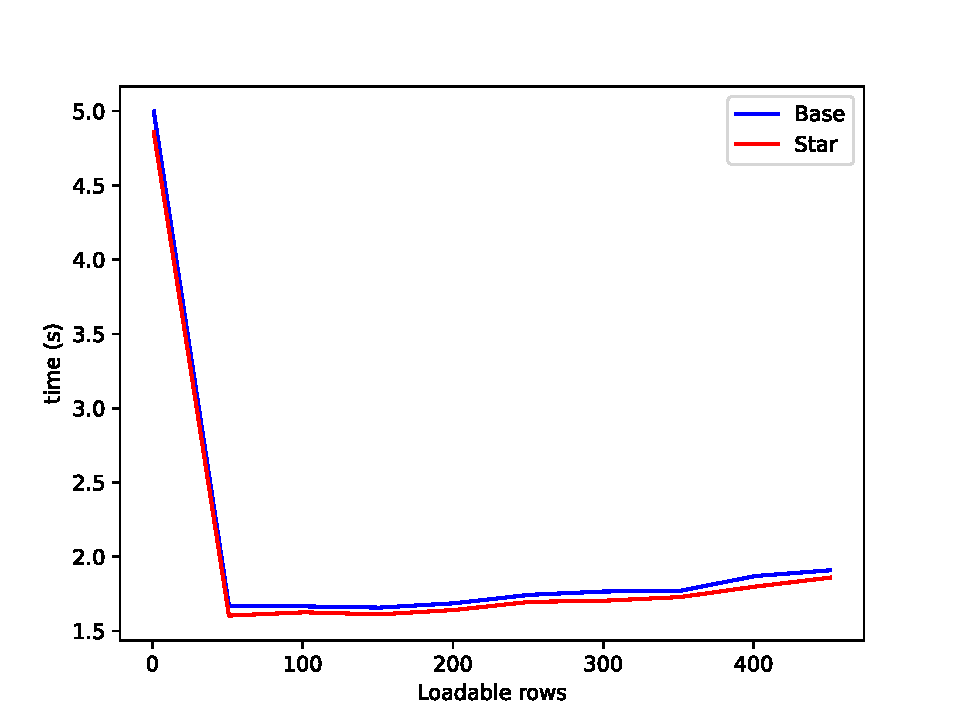
\includegraphics[width=0.75\textwidth]{loadable_rows_time_diff.pdf}
        % \caption{}
        \label{fig:load_portions_a}
    \end{figure}
\end{frame}

\begin{frame}
    \begin{figure}
        \centering
        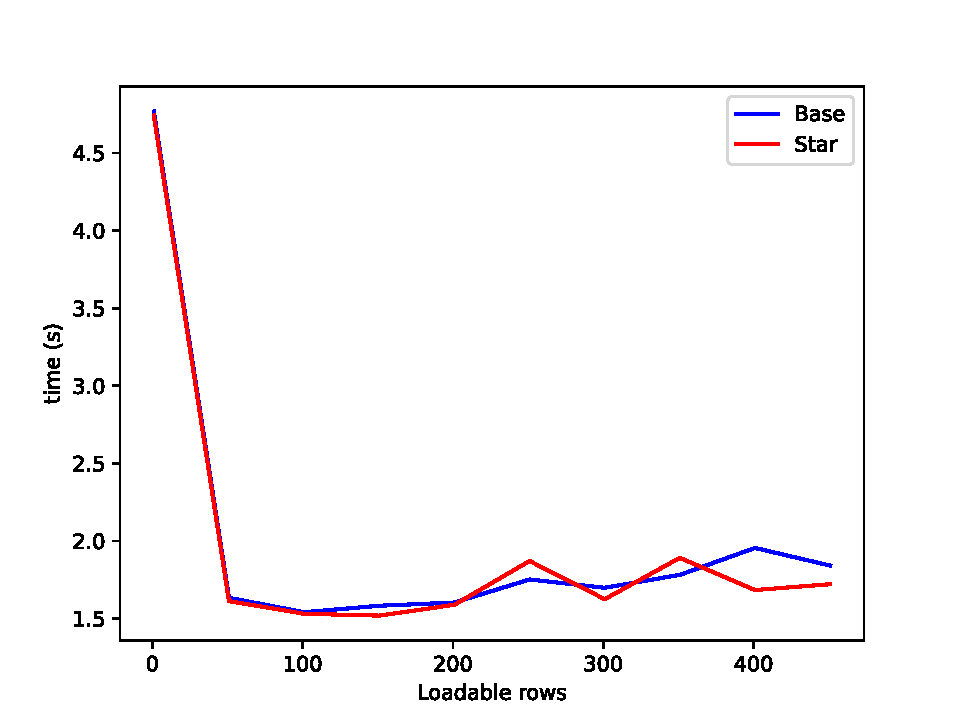
\includegraphics[width=0.75\textwidth]{loadable_rows_time_diff_rev.pdf}
        % \caption{}
        \label{fig:load_portions_b}
    \end{figure}
\end{frame}

\begin{frame}
I manually tried to test the behaviour of the algorithm for
different dimensions of the chunk on a larger problem (1000 rows
and 15 columns) and 
% when loading 1 row at a time the algorithm takes 24.5 seconds, 
% when loading 2 rows it takes 15.3 seconds,
% when loading 3 rows it takes 12.3 seconds,
% when loading 5 rows it takes 9.7 seconds, 
% when loading 10 rows it takes 7.9 seconds,
% when loading 20 rows it takes 6.9 seconds,
% when loading 50 rows it takes 6.5 seconds,
% when loading 100 rows it takes 6.5 seconds,
% when loading 400 rows it takes 6.6 seconds.
\begin{itemize}
    \item when loading 1 row at a time the algorithm takes 24.5 seconds;
    \item when loading 2 rows it takes 15.3 seconds;
    \item when loading 3 rows it takes 12.3 seconds;
    \item when loading 5 rows it takes 9.7 seconds;
    \item when loading 10 rows it takes 7.9 seconds;
    \item when loading 20 rows it takes 6.9 seconds;
    \item when loading 50 rows it takes 6.5 seconds;
    \item when loading 100 rows it takes 6.5 seconds;
    \item when loading 400 rows it takes 6.6 seconds;
    \item when loading 900 rows it takes 7.1 seconds.
    \item when loading 1000 rows it takes 7.6 seconds
\end{itemize}
\end{frame}

\begin{frame}{EC wrapper}
    In the following slides the mechanism wrapping the EC algorithm
    is presented. 
    The idea is to load a portion of the matrix A, execute the EC algorithm
    and store the solutions found in a set, then load the next portion of
    the matrix A, execute the EC algorithm and grow the set of solutions.
    The important thing to keep in mind is that when the algorithm 
    is executing on a portion of the matrix A, say from row $i$ to row $j$,
    the rows from $0$ to $i-1$ are not immediately available, they will
    be read from within the EC algorithm, again in portions.
    % color for offset -> #FF1A1A
    % color for reading offset -> #1A40FF
    This explains the need for two variables:
    \textcolor{offset}{offset} and the \textcolor{reading_offset}{reading offset}
    (the same colors will be used in the schema and the animation to follow.)
\end{frame}

\begin{frame}{}
    \begin{itemize}
        \item \textcolor{offset}{offset} is the index of the first row of the portion
            of the matrix A that has been passed to the EC algorithm from outside
        \item \textcolor{reading_offset}{reading offset} is the index of the first row of the portion
            of the matrix A that is being read by the EC algorithm,
            reading offset will always start from 0 and will be incremented until
            the rows are read from 0 to the last row of the portion of the matrix A 
            that has been passed to the EC algorithm from outside.
    \end{itemize}
\end{frame}

\begin{frame}{}
    \begin{algorithmic}[1]
        % \Function{CalculateFactorial}{$n$}
        %     \If {$n \leq 1$}
        %         \State \Return 1
        %     \Else
        %         \State $result \gets 1$
        %         \For{$i \gets 1$ to $n$}
        %             \State $result \gets result \times i$
        %         \EndFor
        %         \State \Return $result$
        %     \EndIf
        % \EndFunction
        % \State $x \gets 5$
        % \State $y \gets \Call{CalculateFactorial}{x}$
        % \State \textbf{print} $y$
        \Function{IncrementalExactCover}{$filename$}
            \State $rows \gets \Call{GetRows}{filename}$
            \State $columns \gets \Call{GetColumns}{filename}$
            \State $B \gets \Call{zeros}{rows, columns}$
            \State $COV \gets \Call{set}{\emptyset}$
            \State $offset \gets 0$
            \While{true}
                \State $A \gets \Call{GetA}{filename, offset, loadableRows}$
                % If A is empty, break
                \If{$A$ is empty}
                    \State \textbf{break}
                \EndIf
                \State \Call{EC}{$A$, $B$, $COV$, $offset$, $filename$, $loadableRows$}
            \EndWhile
            \State \Return $COV$
        \EndFunction
    \end{algorithmic}
\end{frame}

% \begin{frame}{}
%     \begin{algorithmic}[1]
%         \Function{IncrementalProcess}{$A$, $B$, $COV$, $offset$, $filename$, $loadable\_rows$}
%             \State $new\_COV$ = \Call{EC}{$A$, $B$, $offset$, $filename$, $loadable\_rows$}
%             \State $COV \gets COV \cup new\_COV$
%         \EndFunction
%     \end{algorithmic}
% \end{frame}

\begin{frame}{}
    \begin{algorithmic}[1]
        \Function{EC}{$A$, $B$, $COV$, $offset$, $filename$, $loadableRows$}
            \State $N \gets \Call{rows}{A}$ \Comment{Number of rows of A}
            \State $M \gets \Call{columns}{A}$ \Comment{Number of columns of A}
            \State $COV \gets \Call{set}{\emptyset}$
            \State $reading\_offset \gets 0$
            \State $new\_COV \gets \Call{EC\_plus}{A, B, offset, reading\_offset, COV, rows, columns, loadable\_rows}$
            \State \Return $new\_COV$
        \EndFunction
    \end{algorithmic}
\end{frame}


\begin{frame}{}
    \begin{figure}
        \centering
        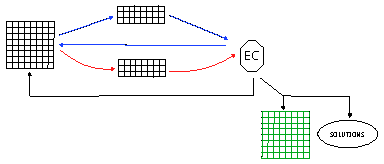
\includegraphics[width=0.75\textwidth]{partial_loading_mech.pdf}
        \label{fig:partial_loading_mech}
    \end{figure}
\end{frame}

\begin{frame}{}
    \begin{figure}
        \centering
        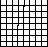
\includegraphics[width=0.45\textwidth]{grid_black.pdf}
        % \caption{}
        \label{fig:grid_black}
    \end{figure}
\end{frame}

\begin{frame}{}
    \begin{table}
        \centering
        \begin{tabular}{|c|c|}
            \hline
            Offset & Reading offset \\
            \hline
            0 & 0 \\
            \hline
        \end{tabular}
    \end{table}
    \begin{figure}
        \centering
        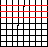
\includegraphics[width=0.45\textwidth]{grid_3r_1.pdf}
        % \caption{}
        \label{fig:grid_3r_1}
    \end{figure}
\end{frame}

\begin{frame}{}
    \begin{table}
        \centering
        \begin{tabular}{|c|c|}
            \hline
            Offset & Reading offset \\
            \hline
            0 & 0 \\
            \hline
        \end{tabular}
    \end{table}
    \begin{figure}
        \centering
        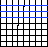
\includegraphics[width=0.45\textwidth]{grid_3r_1_ro_1.pdf}
        % \caption{}
        \label{fig:grid_3r_1_ro_1}
    \end{figure}
\end{frame}

\begin{frame}{}
    \begin{table}
        \centering
        \begin{tabular}{|c|c|}
            \hline
            Offset & Reading offset \\
            \hline
            3 & 0 \\
            \hline
        \end{tabular}
    \end{table}
    \begin{figure}
        \centering
        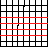
\includegraphics[width=0.45\textwidth]{grid_3r_2.pdf}
        % \caption{}
        \label{fig:grid_3r_2}
    \end{figure}
\end{frame}

\begin{frame}{}
    \begin{table}
        \centering
        \begin{tabular}{|c|c|}
            \hline
            Offset & Reading offset \\
            \hline
            3 & 0 \\
            \hline
        \end{tabular}
    \end{table}
    \begin{figure}
        \centering
        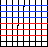
\includegraphics[width=0.45\textwidth]{grid_3r_2_ro_1.pdf}
        % \caption{}
        \label{fig:grid_3r_2_ro_1}
    \end{figure}
\end{frame}

\begin{frame}{}
    \begin{table}
        \centering
        \begin{tabular}{|c|c|}
            \hline
            Offset & Reading offset \\
            \hline
            3 & 3 \\
            \hline
        \end{tabular}
    \end{table}
    \begin{figure}
        \centering
        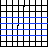
\includegraphics[width=0.45\textwidth]{grid_3r_2_ro_2.pdf}
        % \caption{}
        \label{fig:grid_3r_2_ro_2}
    \end{figure}
\end{frame}

\begin{frame}{}
    \begin{table}
        \centering
        \begin{tabular}{|c|c|}
            \hline
            Offset & Reading offset \\
            \hline
            6 & 0 \\
            \hline
        \end{tabular}
    \end{table}
    \begin{figure}
        \centering
        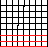
\includegraphics[width=0.45\textwidth]{grid_3r_3.pdf}
        % \caption{}
        \label{fig:grid_3r_3}
    \end{figure}
\end{frame}

\begin{frame}{}
    \begin{table}
        \centering
        \begin{tabular}{|c|c|}
            \hline
            Offset & Reading offset \\
            \hline
            6 & 0 \\
            \hline
        \end{tabular}
    \end{table}
    \begin{figure}
        \centering
        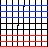
\includegraphics[width=0.45\textwidth]{grid_3r_3_ro_1.pdf}
        % \caption{}
        \label{fig:grid_3r_3_ro_1}
    \end{figure}
\end{frame}

\begin{frame}{}
    \begin{table}
        \centering
        \begin{tabular}{|c|c|}
            \hline
            Offset & Reading offset \\
            \hline
            6 & 3 \\
            \hline
        \end{tabular}
    \end{table}
    \begin{figure}
        \centering
        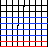
\includegraphics[width=0.45\textwidth]{grid_3r_3_ro_2.pdf}
        % \caption{}
        \label{fig:grid_3r_3_ro_2}
    \end{figure}
\end{frame}

\begin{frame}{}
    \begin{table}
        \centering
        \begin{tabular}{|c|c|}
            \hline
            Offset & Reading offset \\
            \hline
            6 & 6 \\
            \hline
        \end{tabular}
    \end{table}
    \begin{figure}
        \centering
        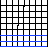
\includegraphics[width=0.45\textwidth]{grid_3r_3_ro_3.pdf}
        % \caption{}
        \label{fig:grid_3r_3_ro_3}
    \end{figure}
\end{frame}

\end{document}